\section{Site cost estimation}

In order to estimate the feasibility of possible computing models in
the future of LHC, some understanding of computing resources costs is
necessary, at a global scale.  This requires an analysis of what
computing expenses are today and what they are likely to be in the
coming years, based on what we have been observing over the last
years.  The main difficulty lies in the fact that various academic
data centers (``sites'') contribute to WLCG, they belong to different
nations with different resource types and costs, different service
levels, funding models, strategies, energy providers and so on. We
tried to understand these differences and provide a set of indicators
that make sense for all sites.

\subsection{\label{sec:sitecost:computing}Computing resource costs}
The first major step of this approach consisted in gathering relevant
indicators related to computing resource and energy costs from the
biggest data centers partcipating in WLCG.  We first focused on the
distributions of CPU, disk and tape cartridge costs for hardware
procured in 2018, as well as the local energy costs.
Figure~\ref{fig:sitecost} represents the anonymized results and
Table~\ref{tab:sitecosts} summarizes the average values and deviation
across sites. Note that due to the special financial model of Site~``F''
tape storage, we removed its contribution from the average tape
cartridge cost value and its standard deviation.

If CPU price is rather homogeneous across sites, the variance in
storage costs is quite important. This effect is due to a larger
diversity in the local storage technology market, and unlike CPU, the
performance is not benchmarked and remains harder to compare across
sites.

In addition to the 2018 purchase costs, we established the evolution
of the purchase costs over the years, per site, although not all sites
could provide relevant data. It is clear that CPU price evolution is
not as fast as expected: all sites oberve a slow down in CPU price
evolution trend, which remains below $-20 \%$ per year in absolute
value.  Concerning disk storage, the picture is rather coherent and
many sites observed a price evolution of about $-15 \%$ per year.  In
the case of tape storage, it is difficult to draw any conclusion from
the observed cost trends across sites: an important change in the tape
and libraries market has been taking place recently, and every site is
in a different situation: we will probably stay on average below the
$-20 \%$ per year for some time.

\begin{figure}[h]
    \subfloat[CPU]{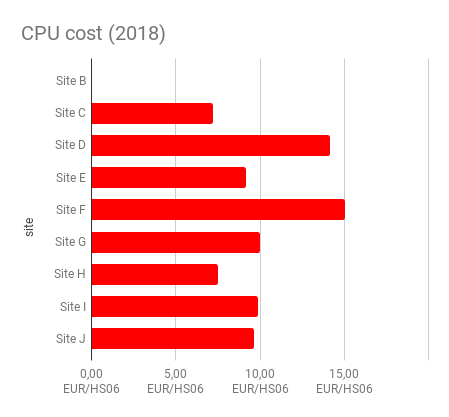
\includegraphics[width = 0.5\textwidth]{CPU_cost.png}}
    \subfloat[Disk]{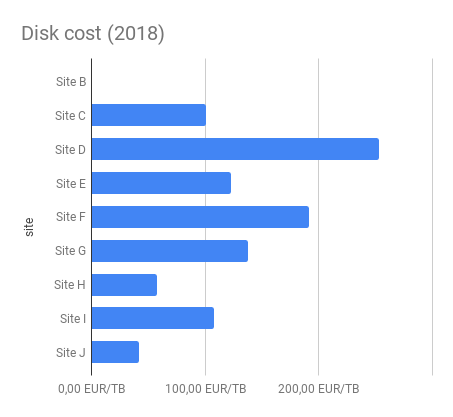
\includegraphics[width = 0.5\textwidth]{Disk_cost.png}} \\
    \subfloat[Tape cartridges]{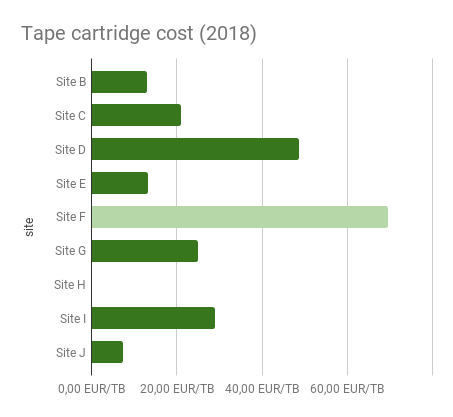
\includegraphics[width = 0.5\textwidth]{Tape_cost.png}}
    \subfloat[Energy]{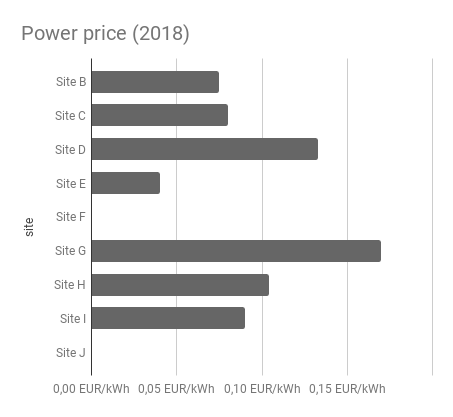
\includegraphics[width = 0.5\textwidth]{Power_price.png}}
    \caption{Add your own figures before compiling}
    \label{fig:sitecost}
\end{figure}

\begin{table}[h]
    \centering
    \caption{Site costs summary (as of 2018) and evolution over the previous years.}
    \label{tab:sitecosts}
    \begin{tabular}{l|cccc}
        \hline
        resource & CPU & disk & cartridge & energy \\\hline
        average purchase cost & 10.3 \euro/HS06 & 126.5 \euro/TB & 12.8 \euro/TB & 0.1 \euro/kWh\\\hline
        standard deviation & 26 \% & 51 \% & 57 \% & 54 \% \\\hline
        average trend & -12 \%/y & -15 \%/y & -14 \%/y & n/a \\\hline
        standard deviation & 37 \% & 20 \% & 43 \% & n/a \\\hline
    \end{tabular}
\end{table}


This set of results provides some insight on the current situation
with respect to resource procurement expenses and their
homogeneity. The trends observed over the last years allow to make a
rough guess on what prices may become in the next years. However, due
to the dispersion of the observed trends across sites, it does not seem
reasonable to try to make predictions for many years ahead.

\subsection{\label{sec:sitecost:tco}TCO}

In this section we address the total cost of ownership (TCO) of a data center.
There is no simple and standard way to calculate a data center TCO, so we use here two different methods which we call
``atomic'' and ``holistic'', based on opposite approaches.

The atomic TCO approach is inspired from the CERN procurement model; it calculate every component needed to build up
a rack with servers, PDUs, switches, uplinks, router, building etc. in association with their respective expenses and lifetime.
The required energy expenses are included, and the human effort expenses to operate a service are also calculated
based on staff expertise and estimated time needed to operate a service.
The results are summarized in Figure~\ref{fig:tco:atomic}.
From the calculation, in both cases IT expenses contribute to most of the atomic TCO, at a level of 70-90~\%.


\begin{figure}[h]
    \subfloat[CPU]{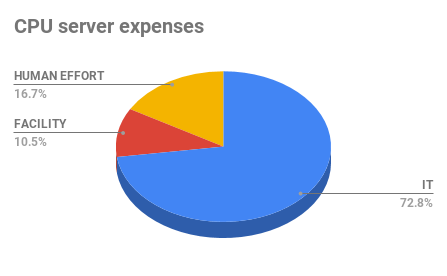
\includegraphics[width = 0.5\textwidth]{atomic_tco_cpu.png}}
    \subfloat[Storage]{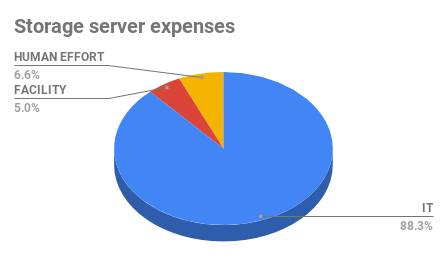
\includegraphics[width = 0.5\textwidth]{atomic_tco_disk.png}}
    \caption{Atomic TCO.}
    \label{fig:tco:atomic}
\end{figure}



The holistic TCO simply consists in taking the average yearly budget spent by a data center.
By definition this includes every expense, those of the atomic TCO plus other sources of expenses, like a tape system,
facility maintenance, developers, project managers, support, administrative staff etc.
In this approach, major expenses that take place occasionally
are distributed over the years according to their expected amortization period.
The calculation of the holistic TCO results in a drastically different picture,
where IT contributes to 30~\% of the budget, the facility about 20 \%, and half of the budget is invested in manpower.

\begin{figure}[h]
    \centering
    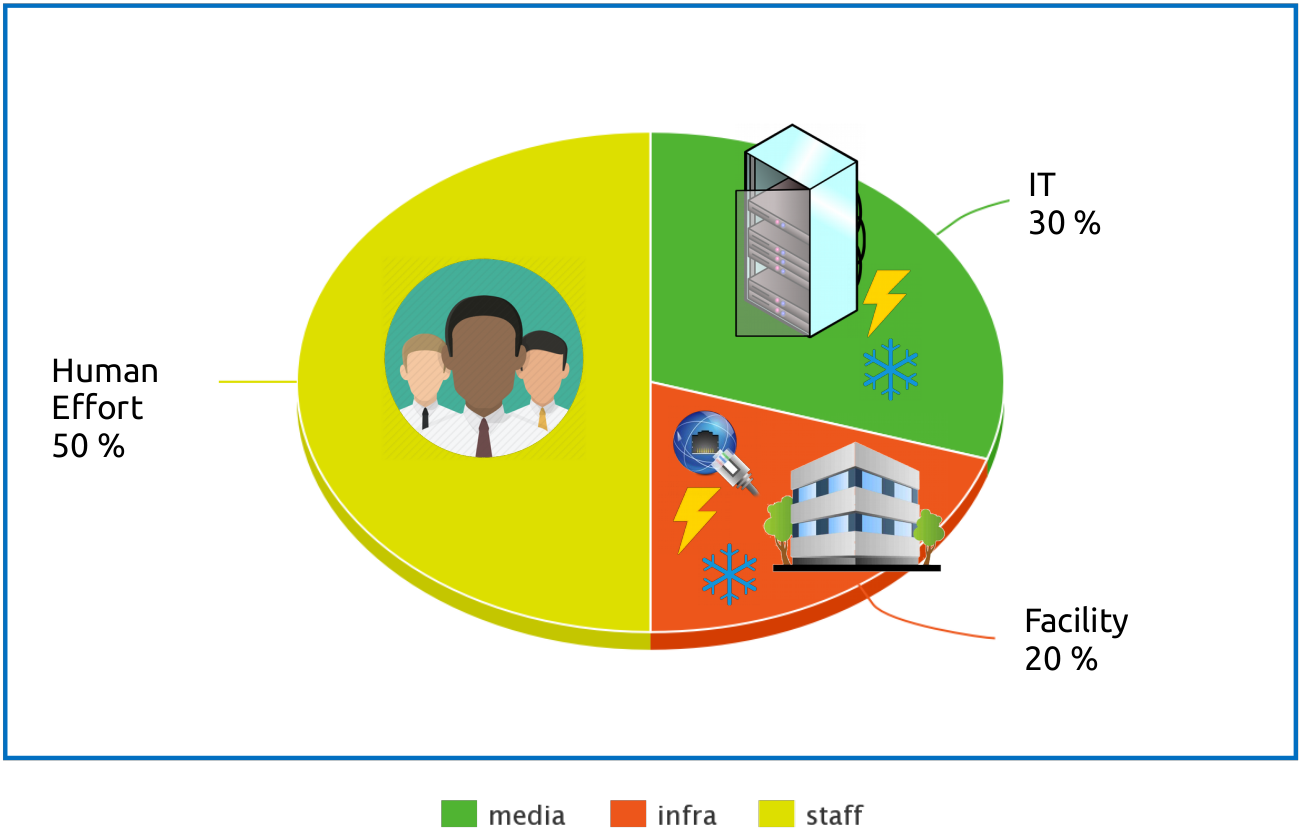
\includegraphics[height=5cm]{holistic_tco.png}
    \caption{Holistic TCO.}
    \label{fig:tco:holistic}
\end{figure}


The difference in the results is mainly explained by the fact that the two considered TCO calculations do not address
the same aspects, especially concerning human effort. Whereas the holistic TCO provides an insight on the breakdown
of expenses in one of the main WLCG data centers, including staff not directly related to the provision of the final service,
the atomic TCO is probably more suited to compute marginal costs when
providing an additional computing or disk-based storage service.



